\section{Linux device and driver model}

\subsection{Introduction}

\begin{frame}{The need for a device model?}
  \begin{itemize}
  \item The Linux kernel runs on a wide range of architectures and
    hardware platforms, and therefore needs to {\bf maximize the
      reusability} of code between platforms.
  \item For example, we want the same {\em USB device driver} to be
    usable on a x86 PC, or an ARM platform, even though the USB
    controllers used on these platforms are different.
  \item This requires a clean organization of the code, with the {\em
      device drivers} separated from the {\em controller drivers}, the
    hardware description separated from the drivers themselves, etc.
  \item This is what the Linux kernel {\bf Device Model} allows, in
    addition to other advantages covered in this section.
  \end{itemize}
\end{frame}

\begin{frame}
  \frametitle{Kernel and Device Drivers}
  \begin{columns}
    \column{0.5\textwidth} In Linux, a driver is always interfacing
    with:
    \begin{itemize}
    \item a {\bf framework} that allows the driver to expose the
      hardware features in a generic way.
    \item a {\bf bus infrastructure}, part of the device model, to
      detect/communicate with the hardware.
    \end{itemize}
    This section focuses on the {\em device model}, while {\em kernel
      frameworks} are covered later in this training.
    \column{0.5\textwidth}
    \includegraphics[height=0.8\textheight]{slides/kernel-device-model/driver-architecture.pdf}
  \end{columns}
\end{frame}

\begin{frame}
  \frametitle{Device Model data structures}
  \begin{itemize}
  \item The {\em device model} is organized around three main data
    structures:
    \begin{itemize}
    \item The \kstruct{bus_type} structure, which represent one type of bus
      (USB, PCI, I2C, etc.)
    \item The \kstruct{device_driver} structure, which represents one driver
      capable of handling certain devices on a certain bus.
    \item The \kstruct{device} structure, which represents one device
      connected to a bus
    \end{itemize}
  \item The kernel uses inheritance to create more specialized
    versions of \kstruct{device_driver} and \kstruct{device}
    for each bus subsystem.
  \item In order to explore the device model, we will
    \begin{itemize}
    \item First look at a popular bus that offers dynamic enumeration,
      the {\em USB bus}
    \item Continue by studying how buses that do not offer dynamic
      enumerations are handled.
    \end{itemize}
  \end{itemize}
\end{frame}

\begin{frame}
  \frametitle{Bus Drivers}
  \begin{itemize}
  \item The first component of the device model is the bus driver
    \begin{itemize}
    \item One bus driver for each type of bus: USB, PCI, SPI, MMC,
      I2C, etc.
    \end{itemize}
  \item It is responsible for
    \begin{itemize}
    \item Registering the bus type (\kstruct{bus_type})
    \item Allowing the registration of adapter drivers (USB
      controllers, I2C adapters, etc.), able to detect the
      connected devices, and providing a communication mechanism with
      the devices
    \item Allowing the registration of device drivers (USB devices,
      I2C devices, PCI devices, etc.), managing the devices
    \item Matching the device drivers against the devices detected by
      the adapter drivers.
    \item Provides an API to both adapter drivers and device drivers
    \item Defining driver and device specific structures, mainly
      \kstruct{usb_driver} and \kstruct{usb_interface}
    \end{itemize}
  \end{itemize}
\end{frame}

\subsection{Example of the USB bus}

\begin{frame}
\frametitle{Example: USB Bus 1/2}
  \begin{center}
    \includegraphics[height=0.8\textheight]{slides/kernel-device-model/usb-bus.pdf}
  \end{center}
\end{frame}

\begin{frame}
  \frametitle{Example: USB Bus 2/2}
  \begin{itemize}
  \item Core infrastructure (bus driver)
    \begin{itemize}
    \item \kdir{drivers/usb/core}
    \item \kstruct{bus_type} is defined in
      \kfile{drivers/usb/core/driver.c} and registered in
      \kfile{drivers/usb/core/usb.c}
    \end{itemize}
  \item Adapter drivers
    \begin{itemize}
    \item \kdir{drivers/usb/host}
    \item For EHCI, UHCI, OHCI, XHCI, and their implementations on
      various systems (Microchip, IXP, Xilinx, OMAP, Samsung, PXA, etc.)
    \end{itemize}
  \item Device drivers
    \begin{itemize}
    \item Everywhere in the kernel tree, classified by their type
    (Example: \kdir{drivers/net/usb})
    \end{itemize}
  \end{itemize}
\end{frame}

\begin{frame}
  \frametitle{Example of Device Driver}
  \begin{itemize}
  \item To illustrate how drivers are implemented to work with the
    device model, we will study the source code of a driver for a USB
    network card
    \begin{itemize}
    \item It is USB device, so it has to be a USB device driver
    \item It exposes a network device, so it has to be a network driver
    \item Most drivers rely on a bus infrastructure (here, USB) and
      register themselves in a framework (here, network)
    \end{itemize}
  \item We will only look at the device driver side, and not the
    adapter driver side
  \item The driver we will look at is \kfile{drivers/net/usb/rtl8150.c}
  \end{itemize}
\end{frame}

\begin{frame}[fragile]
  \frametitle{Device Identifiers}
  \begin{itemize}
  \item Defines the set of devices that this driver can manage, so
    that the USB core knows for which devices this driver should be
    used
  \item The \kfunc{MODULE_DEVICE_TABLE} macro allows \code{depmod}
    (run by \code{make modules_install}) to extract the relationship
    between device identifiers and drivers, so that drivers can be
    loaded automatically by \code{udev}.
    See \code{/lib/modules/$(uname -r)/modules.{alias,usbmap}}
  \end{itemize}
  \begin{block}{}
  \begin{minted}[fontsize=\footnotesize]{c}
static struct usb_device_id rtl8150_table[] = {
    { USB_DEVICE(VENDOR_ID_REALTEK, PRODUCT_ID_RTL8150) },
    { USB_DEVICE(VENDOR_ID_MELCO, PRODUCT_ID_LUAKTX) },
    { USB_DEVICE(VENDOR_ID_MICRONET, PRODUCT_ID_SP128AR) },
    { USB_DEVICE(VENDOR_ID_LONGSHINE, PRODUCT_ID_LCS8138TX) },
    [...]
    {}
};
MODULE_DEVICE_TABLE(usb, rtl8150_table);
  \end{minted}
  \end{block}
\end{frame}

\begin{frame}[fragile]
  \frametitle{Instantiation of usb\_driver}
  \begin{itemize}
  \item \kstruct{usb_driver} is a structure defined by the USB
    core. Each USB device driver must instantiate it, and register
    itself to the USB core using this structure
  \item This structure inherits from \kstruct{device_driver},
    which is defined by the device model.
    \begin{block}{}
  \begin{minted}{c}
static struct usb_driver rtl8150_driver = {
    .name = "rtl8150",
    .probe = rtl8150_probe,
    .disconnect = rtl8150_disconnect,
    .id_table = rtl8150_table,
    .suspend = rtl8150_suspend,
    .resume = rtl8150_resume
};
  \end{minted}
  \end{block}
  \end{itemize}
\end{frame}

\begin{frame}[fragile]
  \frametitle{Driver (Un)Registration}
  \begin{itemize}
  \item When the driver is loaded or unloaded, it must register or
    unregister itself from the USB core
  \item Done using \kfunc{usb_register} and \kfunc{usb_deregister},
    provided by the USB core.
    \begin{block}{}
\begin{minted}[fontsize=\scriptsize]{c}
static int __init usb_rtl8150_init(void)
{
    return usb_register(&rtl8150_driver);
}

static void __exit usb_rtl8150_exit(void)
{
    usb_deregister(&rtl8150_driver);
}

module_init(usb_rtl8150_init);
module_exit(usb_rtl8150_exit);
\end{minted}
\end{block}
\item Note: this code has now been replaced by a shorter
  \kfunc{module_usb_driver} macro call.
  \end{itemize}
\end{frame}

\begin{frame}
  \frametitle{At Initialization}
  \begin{itemize}
  \item The USB adapter driver that corresponds to the USB controller
    of the system registers itself to the USB core
  \item The \ksym{rtl8150} USB device driver registers itself to the USB core
    \begin{center}
      \includegraphics[height=0.4\textheight]{slides/kernel-device-model/usb-registering.pdf}
    \end{center}
  \item The USB core now knows the association between the
    vendor/product IDs of \ksym{rtl8150} and the \kstruct{usb_driver} structure
    of this driver
  \end{itemize}
\end{frame}

\begin{frame}
  \frametitle{When a device is detected}
  \begin{center}
    \includegraphics[width=\textwidth]{slides/kernel-device-model/usb-detection.pdf}
  \end{center}
\end{frame}

\begin{frame}
  \frametitle{Probe Method}
  \begin{itemize}
  \item Invoked {\bf for each device} bound to a driver
  \item The \code{probe()} method receives as argument a structure
    describing the device, usually specialized by the bus
    infrastructure (\kstruct{pci_dev}, \kstruct{usb_interface}, etc.)
  \item This function is responsible for
    \begin{itemize}
    \item Initializing the device, mapping I/O memory, registering the
      interrupt handlers. The bus infrastructure provides methods to
      get the addresses, interrupt numbers and other device-specific
      information.
    \item Registering the device to the proper kernel framework, for
      example the network infrastructure.
    \end{itemize}
  \end{itemize}
\end{frame}

\begin{frame}[fragile]
\frametitle{Example: probe() and disconnect() methods}
\begin{columns}
  \column{0.5\textwidth}
    \begin{block}{}
    \begin{minted}[fontsize=\tiny]{c}
static int rtl8150_probe(struct usb_interface *intf,
    const struct usb_device_id *id)
{
    rtl8150_t *dev;
    struct net_device *netdev;

    netdev = alloc_etherdev(sizeof(rtl8150_t));
    [...]
    dev = netdev_priv(netdev);
    tasklet_init(&dev->tl, rx_fixup, (unsigned long)dev);
    spin_lock_init(&dev->rx_pool_lock);
    [...]
    netdev->netdev_ops = &rtl8150_netdev_ops;
    alloc_all_urbs(dev);
    [...]
    usb_set_intfdata(intf, dev);
    SET_NETDEV_DEV(netdev, &intf->dev);
    register_netdev(netdev);

    return 0;
}
    \end{minted}
    \end{block}
  \column{0.5\textwidth}
    \begin{block}{}
    \begin{minted}[fontsize=\tiny]{c}
static void rtl8150_disconnect(struct usb_interface *intf)
{
        rtl8150_t *dev = usb_get_intfdata(intf);

        usb_set_intfdata(intf, NULL);
        if (dev) {
                set_bit(RTL8150_UNPLUG, &dev->flags);
                tasklet_kill(&dev->tl);
                unregister_netdev(dev->netdev);
                unlink_all_urbs(dev);
                free_all_urbs(dev);
                free_skb_pool(dev);
                if (dev->rx_skb)
                        dev_kfree_skb(dev->rx_skb);
                kfree(dev->intr_buff);
                free_netdev(dev->netdev);
        }
}
    \end{minted}
    \end{block}
\end{columns}
\vfill
Source: \kfile{drivers/net/usb/rtl8150.c}
\end{frame}

\begin{frame}
  \frametitle{The Model is Recursive}
  \begin{center}
    \includegraphics[height=0.8\textheight]{slides/kernel-device-model/recursive-model.pdf}
  \end{center}
\end{frame}

\subsection{Platform drivers}

\begin{frame}{Non-discoverable buses}
  \begin{itemize}
  \item On embedded systems, devices are often not connected through a
    bus allowing enumeration, hotplugging, and providing unique
    identifiers for devices.
  \item For example, the devices on I2C buses or SPI buses, or the
    devices directly part of the system-on-chip.
  \item However, we still want all of these devices to be part of the
    device model.
  \item Such devices, instead of being dynamically detected, must be
    statically described in either:
    \begin{itemize}
    \item The kernel source code
    \item The {\em Device Tree}, a hardware description file used on
      some architectures.
    \item BIOS ACPI tables (x86/PC architecture)
    \end{itemize}
  \end{itemize}
\end{frame}

\begin{frame}{Platform devices}
  \begin{itemize}
  \item Amongst the non-discoverable devices, a huge family are the
    devices that are directly part of a system-on-chip: UART
    controllers, Ethernet controllers, SPI or I2C controllers, graphic
    or audio devices, etc.
  \item In the Linux kernel, a special bus, called the {\bf platform
      bus} has been created to handle such devices.
  \item It supports {\bf platform drivers} that handle {\bf platform
      devices}.
  \item It works like any other bus (USB, PCI), except that devices
    are enumerated statically instead of being discovered dynamically.
  \end{itemize}
\end{frame}

\begin{frame}[fragile]
  \frametitle{Implementation of a Platform Driver (1)}
  The driver implements a \kstruct{platform_driver}
  structure (example taken from \kfile{drivers/tty/serial/imx.c},
  simplified)
  \begin{block}{}
  \begin{minted}[fontsize=\scriptsize]{c}
static struct platform_driver serial_imx_driver = {
        .probe          = serial_imx_probe,
        .remove         = serial_imx_remove,
        .id_table       = imx_uart_devtype,
        .driver         = {
                .name   = "imx-uart",
                .of_match_table = imx_uart_dt_ids,
                .pm     = &imx_serial_port_pm_ops,
        },
};
\end{minted}
\end{block}
\end{frame}


\begin{frame}[fragile]
  \frametitle{Implementation of a Platform Driver (2)}
  ... and registers its driver to the platform driver infrastructure
  \begin{block}{}
  \begin{minted}[fontsize=\scriptsize]{c}
static int __init imx_serial_init(void) {
    ret = platform_driver_register(&serial_imx_driver);
}

static void __exit imx_serial_cleanup(void) {
    platform_driver_unregister(&serial_imx_driver);
}
  \end{minted}
\end{block}
Most drivers actually use the \kfunc{module_platform_driver}
macro when they do nothing special in \code{init()} and \code{exit()} functions.
\end{frame}

\begin{frame}[fragile]
  \frametitle{Platform Device Instantiation: old style (1/2)}
  \begin{itemize}
  \item As platform devices cannot be detected dynamically, they are
    defined statically
    \begin{itemize}
    \item By direct instantiation of \kstruct{platform_device}
      structures, as done on a few old ARM platforms. Definition done in
      the board-specific or SoC specific code.
    \item By using a \emph{device tree}, as done on Power PC (and on
      most ARM platforms) from which \kstruct{platform_device}
      structures are created
    \end{itemize}
  \item Example on ARM, where the instantiation was done in
    \kfileversion{arch/arm/mach-imx/mx1ads.c}{2.6.30}
    \begin{block}{}
\begin{minted}[fontsize=\scriptsize]{c}
static struct platform_device imx_uart1_device = {
    .name = "imx-uart",
    .id = 0,
    .num_resources = ARRAY_SIZE(imx_uart1_resources),
    .resource = imx_uart1_resources,
    .dev = {
         .platform_data = &uart_pdata,
    }
};
\end{minted}
\end{block}
\end{itemize}
\end{frame}

\begin{frame}[fragile]
  \frametitle{Platform device instantiation: old style (2/2)}
  \begin{itemize}
  \item The device was part of a list
    \begin{block}{}
  \begin{minted}[fontsize=\scriptsize]{c}
static struct platform_device *devices[] __initdata = {
    &cs89x0_device,
    &imx_uart1_device,
    &imx_uart2_device,
};
  \end{minted}
  \end{block}
  \item And the list of devices was added to the system during
    board initialization
    \begin{block}{}
  \begin{minted}[fontsize=\scriptsize]{c}
static void __init mx1ads_init(void)
{
    [...]
    platform_add_devices(devices, ARRAY_SIZE(devices));
}

MACHINE_START(MX1ADS, "Freescale MX1ADS")
    [...]
    .init_machine = mx1ads_init,
MACHINE_END
  \end{minted}
  \end{block}
  \end{itemize}
\end{frame}

\begin{frame}
  \frametitle{The Resource Mechanism}
  \begin{itemize}
  \item Each device managed by a particular driver typically uses
    different hardware resources: addresses for the I/O registers, DMA
    channels, IRQ lines, etc.
  \item Such information can be represented using
    \kstruct{resource}, and an array of \kstruct{resource} is
    associated to a \kstruct{platform_device}
  \item Allows a driver to be instantiated for multiple devices
    functioning similarly, but with different addresses, IRQs, etc.
  \end{itemize}
\end{frame}

\begin{frame}[fragile]
  \frametitle{Declaring resources (old style)}
  \begin{block}{}
  \begin{minted}[fontsize=\footnotesize]{c}
static struct resource imx_uart1_resources[] = {
    [0] = {
        .start = 0x00206000,
        .end = 0x002060FF,
        .flags = IORESOURCE_MEM,
    },
    [1] = {
        .start = (UART1_MINT_RX),
        .end = (UART1_MINT_RX),
        .flags = IORESOURCE_IRQ,
    },
};
\end{minted}
\end{block}
\end{frame}

\begin{frame}[fragile]
  \frametitle{Using Resources (old style)}
  \begin{itemize}
  \item When a \kstruct{platform_device} was added to the system using
    \kfunc{platform_add_devices}, the \code{probe()} method of the
    platform driver was called
  \item This method is responsible for initializing the hardware,
    registering the device to the proper framework (in our case, the
    serial driver framework)
  \item The platform driver has access to the I/O resources:
    \begin{block}{}
  \begin{minted}[fontsize=\footnotesize]{c}
res = platform_get_resource(pdev, IORESOURCE_MEM, 0);
base = ioremap(res->start, PAGE_SIZE);
sport->rxirq = platform_get_irq(pdev, 0);
  \end{minted}
  \end{block}
  \end{itemize}
\end{frame}

\begin{frame}
  \frametitle{platform\_data Mechanism (old style)}
  \begin{itemize}
  \item In addition to the well-defined resources, many drivers
    require driver-specific information for each platform device
  \item Such information could be passed using the \code{platform_data}
    field of \kstruct{device} (from which
    \kstruct{platform_device} inherits)
  \item As it is a \code{void *} pointer, it could be used to pass any
    type of information.
    \begin{itemize}
    \item Typically, each driver defines a structure to pass
      information through \kstruct{platform_data}
    \end{itemize}
  \end{itemize}
\end{frame}

\begin{frame}[fragile]
  \frametitle{platform\_data example 1/2}
  \begin{itemize}
  \item The i.MX serial port driver defines the following structure to
    be passed through \kstruct{platform_data}
    \begin{block}{}
  \begin{minted}[fontsize=\footnotesize]{c}
struct imxuart_platform_data {
    int (*init)(struct platform_device *pdev);
    void (*exit)(struct platform_device *pdev);
    unsigned int flags;
    void (*irda_enable)(int enable);
    unsigned int irda_inv_rx:1;
    unsigned int irda_inv_tx:1;
    unsigned short transceiver_delay;
};
  \end{minted}
  \end{block}
  \item The MX1ADS board code instantiated such a structure
    \begin{block}{}
  \begin{minted}[fontsize=\footnotesize]{c}
static struct imxuart_platform_data uart1_pdata = {
    .flags = IMXUART_HAVE_RTSCTS,
};
  \end{minted}
  \end{block}
  \end{itemize}
\end{frame}

\begin{frame}[fragile]
  \frametitle{platform\_data Example 2/2}
  \begin{itemize}
  \item The \code{uart_pdata} structure was associated to the
    \kstruct{platform_device} structure in the MX1ADS board file (the
    real code was slightly more complicated)
    \begin{block}{}
  \begin{minted}[fontsize=\scriptsize]{c}
struct platform_device mx1ads_uart1 = {
    .name = "imx-uart",
    .dev {
         .platform_data = &uart1_pdata,
    },
    .resource = imx_uart1_resources,
    [...]
};
  \end{minted}
  \end{block}
  \item The driver can access the platform data:
    \begin{block}{}
  \begin{minted}[fontsize=\scriptsize]{c}
static int serial_imx_probe(struct platform_device *pdev)
{
    struct imxuart_platform_data *pdata;
    pdata = pdev->dev.platform_data;
    if (pdata && (pdata->flags & IMXUART_HAVE_RTSCTS))
        sport->have_rtscts = 1;
    [...]
  \end{minted}
  \end{block}
\end{itemize}
\end{frame}

\begin{frame}
  \frametitle{Device Tree}
  \begin{itemize}
  \item On many embedded architectures, manual instantiation of
    platform devices was considered to be too verbose and not easily
    maintainable.
  \item Such architectures are moving, or have moved, to use the {\em
      Device Tree}.
  \item It is a {\bf tree of nodes} that models the hierarchy of
    devices in the system, from the devices inside the processor to
    the devices on the board.
  \item Each node can have a number of {\bf properties} describing
    various properties of the devices: addresses, interrupts, clocks,
    etc.
  \item At boot time, the kernel is given a compiled version, the {\bf
      Device Tree Blob}, which is parsed to instantiate all the
    devices described in the DT.
  \item On ARM, they are located in \kdir{arch/arm/boot/dts}.
  \end{itemize}
\end{frame}

\begin{frame}[fragile]
  \frametitle{Device Tree example}
  \begin{block}{}
\begin{minted}[fontsize=\small]{perl}
uart0: serial@44e09000 {
        compatible = "ti,omap3-uart";
        ti,hwmods = "uart1";
        clock-frequency = <48000000>;
        reg = <0x44e09000 0x2000>;
        interrupts = <72>;
        status = "disabled";
};
  \end{minted}
  \end{block}
  \normalsize
  \begin{itemize}
  \item \code{serial@44e09000} is the {\bf node name}
  \item \code{uart0} is a {\bf label}, that can be referred to in other
    parts of the DT as \code{&uart0}
  \item other lines are {\bf properties}. Their values are usually
    strings, list of integers, or references to other nodes.
  \end{itemize}
\end{frame}

\begin{frame}
  \frametitle{Device Tree inheritance (1/2)}
  \begin{itemize}
  \item Each particular hardware platform has its own {\em device tree}.
  \item However, several hardware platforms use the same processor,
    and often various processors in the same family share a number of
    similarities.
  \item To allow this, a {\em device tree} file can include another
    one. The trees described by the including file overlays the tree
    described by the included file. This can be done:
    \begin{itemize}
       \item Either by using the \code{/include/} statement
         provided by the Device Tree language.
       \item Either by using the {\usebeamercolor[fg]{code}\tt
         \#include} statement, which requires calling the C
         preprocessor before parsing the Device Tree.
    \end{itemize}
    Linux currently uses either one technique or the other,
    (different from one ARM subarchitecture to another, for example).
  \end{itemize}
\end{frame}

\begin{frame}
  \frametitle{Device Tree inheritance (2/2)}
  \begin{center}
    \includegraphics[height=0.8\textheight]{slides/kernel-device-model/dt-inheritance.pdf}
  \end{center}
\end{frame}

\begin{frame}[fragile]
  \frametitle{Device Tree: {\tt compatible} string}
  \begin{itemize}
  \item With the {\em device tree}, a {\em device} is bound to the
    corresponding {\em driver} using the {\bf compatible} string.
  \item The \code{of_match_table} field of \kstruct{device_driver}
    lists the compatible strings supported by the driver.
    \begin{block}{}
  \begin{minted}[fontsize=\tiny]{c}
#if defined(CONFIG_OF)
static const struct of_device_id omap_serial_of_match[] = {
        { .compatible = "ti,omap2-uart" },
        { .compatible = "ti,omap3-uart" },
        { .compatible = "ti,omap4-uart" },
        {},
};
MODULE_DEVICE_TABLE(of, omap_serial_of_match);
#endif
static struct platform_driver serial_omap_driver = {
        .probe          = serial_omap_probe,
        .remove         = serial_omap_remove,
        .driver         = {
                .name   = DRIVER_NAME,
                .pm     = &serial_omap_dev_pm_ops,
                .of_match_table = of_match_ptr(omap_serial_of_match),
        },
};
\end{minted}
\end{block}
  \end{itemize}
\end{frame}

\begin{frame}
  \frametitle{Device Tree Resources}
  \begin{itemize}
  \item The drivers will use the same mechanism that we saw previously
    to retrieve basic information: interrupts numbers, physical
    addresses, etc.
  \item The available resources list will be built up by the kernel at
    boot time from the device tree, so that you don't need to make any
    unnecessary lookups to the DT when loading your driver.
  \item Any additional information will be specific to a driver or
    the class it belongs to, defining the {\em bindings}
  \end{itemize}
\end{frame}

\begin{frame}{Device Tree bindings}
  \begin{itemize}
  \item The compatible string and the associated properties define
    what is called a {\em device tree binding}.
  \item {\em Device tree bindings} are all documented in
    \kerneldoctext{devicetree/bindings}.
  \item Since the Device Tree is normally part of the kernel ABI, the
    {\em bindings} must remain compatible over time.
    \begin{itemize}
    \item A new kernel must be capable of using an old Device Tree.
    \item This requires a very careful design of the bindings. They
      are all reviewed on the \code{devicetree@vger.kernel.org}
      mailing list.
    \item See Thomas Petazzoni's presentation on this topic:
          {\em Device Tree as a stable ABI: a fairy tale?}
	  (\url{http://bit.ly/1U1tYkT}).
    \end{itemize}
  \item A Device Tree binding should contain only a {\em description
      of the hardware} and not {\em configuration}.
    \begin{itemize}
    \item An interrupt number can be part of the Device Tree as it
      describes the hardware.
    \item But not whether DMA should be used for a device or not,
      as it is a configuration choice.
    \end{itemize}
  \end{itemize}
\end{frame}

\begin{frame}
  \frametitle{sysfs}
  \begin{itemize}
  \item The bus, device, drivers, etc. structures are internal to the
    kernel
  \item The \code{sysfs} virtual filesystem offers a mechanism to
    export such information to user space
  \item Used for example by \code{udev} to provide automatic module loading,
    firmware loading, mounting of external media, etc.
  \item \code{sysfs} is usually mounted in \code{/sys}
    \begin{itemize}
    \item \code{/sys/bus/} contains the list of buses
    \item \code{/sys/devices/} contains the list of devices
    \item \code{/sys/class} enumerates devices by class (\code{net},
      \code{input}, \code{block}...), whatever the bus they are connected
      to. Very useful!
    \end{itemize}
  \item Take your time to explore \code{/sys} on your workstation.
  \end{itemize}
\end{frame}

\begin{frame}
  \frametitle{References}
  \begin{columns}
    \column{0.5\textwidth}
       \begin{itemize}
       \item Device Tree for Dummies, Thomas Petazzoni (Apr. 2014):
             \url{http://j.mp/1jQU6NR}
       \item Kernel documentation
         \begin{itemize}
         \item \kerneldoctext{driver-model/}
         \item \kerneldoctext{devicetree/}
         \item \kerneldoctext{filesystems/sysfs.txt}
         \end{itemize}
      \item \url{http://devicetree.org}
       \item The kernel source code
         \begin{itemize}
         \item Full of examples of other drivers!
         \end{itemize}
       \end{itemize}
    \column{0.5\textwidth}
    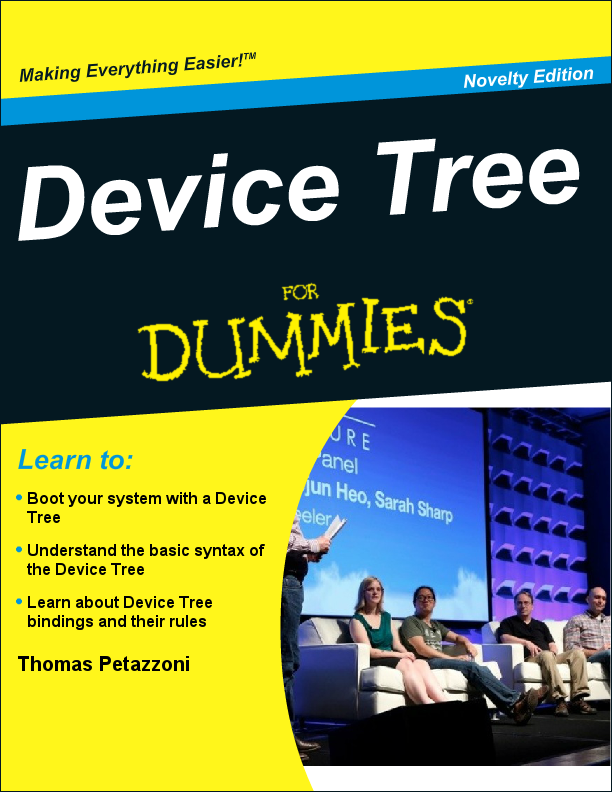
\includegraphics[height=0.8\textheight]{slides/kernel-device-model/device-tree-for-dummies.png}
  \end{columns}
\end{frame}

